\section{Dynamic Behavior and Control}

Tilting Narrow Track Vehicles (NTVs) with a high center of mass (CoM) are inherently unstable, necessitating active stabilization to remain upright and controllable. Due to time constraints, a full dynamic controller is beyond the scope of this work. Instead, we demonstrate the viability of steady-state stabilization using a tuned PID controller to maintain balance during straight-line travel and constant-radius turns. The primary goal is to compare the dynamic response of multiple design variants, specifically 3-wheel versus 4-wheel layouts, and rotational versus linear tilt arm mechanisms, under two representative conditions. This results in a total of 8 simulated scenarios. Each simulation is treated as a steady-state configuration, with basic PID control used to stabilize the lean angle. While this does not capture transient or disturbance responses, it is sufficient to evaluate geometry-dependent trends and identify promising configurations for further development.


\subsection{Methodology}

The simulation framework was built using PyBullet, a real-time physics engine. Each vehicle configuration was modeled using a URDF file that specifies link geometry, mass distribution, and joint constraints. Four base configurations were created by combining two platform layouts (three-wheel and four-wheel) with two leaning mechanisms (pivot-based and linear-guided). Each of these was simulated under two scenarios: straight-line motion and constant-radius turning, yielding eight unique scenarios. The straight line scenario occurred on a bumpy surface, while the Curved scenario operated on a flat surface.

For each configuration, the lean angle was controlled via a custom PID controller implemented in the simulation loop. The system was initialized at rest and brought to a constant velocity. For turning scenarios, a fixed-radius turn was imposed by constraining the trajectory. The controller was responsible for adjusting the lean angle to balance centrifugal forces during turning or gravitational instability during straight-line motion.

All simulations recorded joint states (position, velocity, acceleration) and key global metrics such as vehicle lean angle, lateral deviation, and applied control torque. Screenshots of each configuration were captured to document visual differences and posture under dynamic conditions.

\subsection{Implementation}

Each vehicle model is defined using a modular URDF structure, with separate subtrees for chassis, suspension, and lean mechanism. The joint-level PID controller operates within the PyBullet simulation loop at a frequency of 240 Hz. The control law follows:

\[
\tau = K_p(\theta_{\text{desired}} - \theta) + K_d(\dot{\theta}_{\text{desired}} - \dot{\theta}) + K_i \int (\theta_{\text{desired}} - \theta) \, dt
\]

where $\tau$ is the control torque, $\theta$ is the lean joint state, and $\dot{\theta}$ is its velocity. Gains $K_p$, $K_i$, and $K_d$ were manually tuned for each configuration to achieve stable convergence and minimize oscillation.

Data was logged for plotting and post-processing. Camera control was implemented to enable 3D inspection of vehicle motion and stability during runtime, facilitating visual validation of lean behavior and dynamic posture. The figure \ref{fig:actuator-configs} show how the different configuration were implemented in pybullet. The Base mass was set to 100 [kg] while the wheel and segment mass were set to 1 [kg] to emphasize the high CoM.

\newpage

\begin{figure}[h!]
    \centering
    \begin{subfigure}[b]{0.45\linewidth}
        \centering
        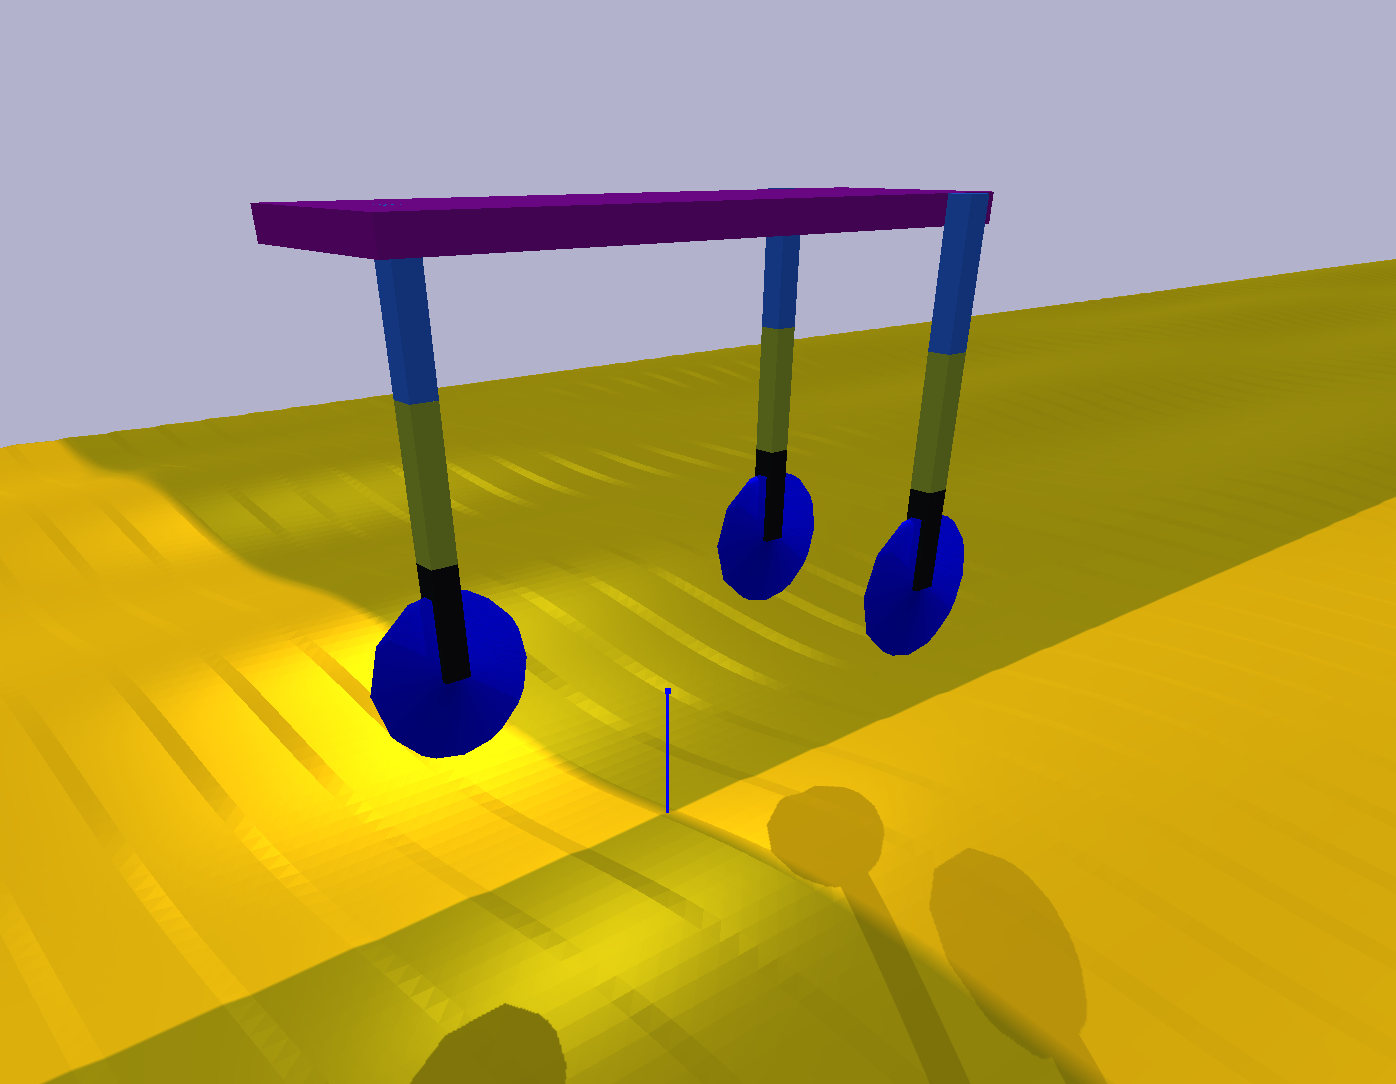
\includegraphics[width=\linewidth]{Figures/ch8_LinearThreeWheel.png}
        \caption{Three Wheeler With Linear Actuator}
    \end{subfigure}
    \hfill
    \begin{subfigure}[b]{0.45\linewidth}
        \centering
        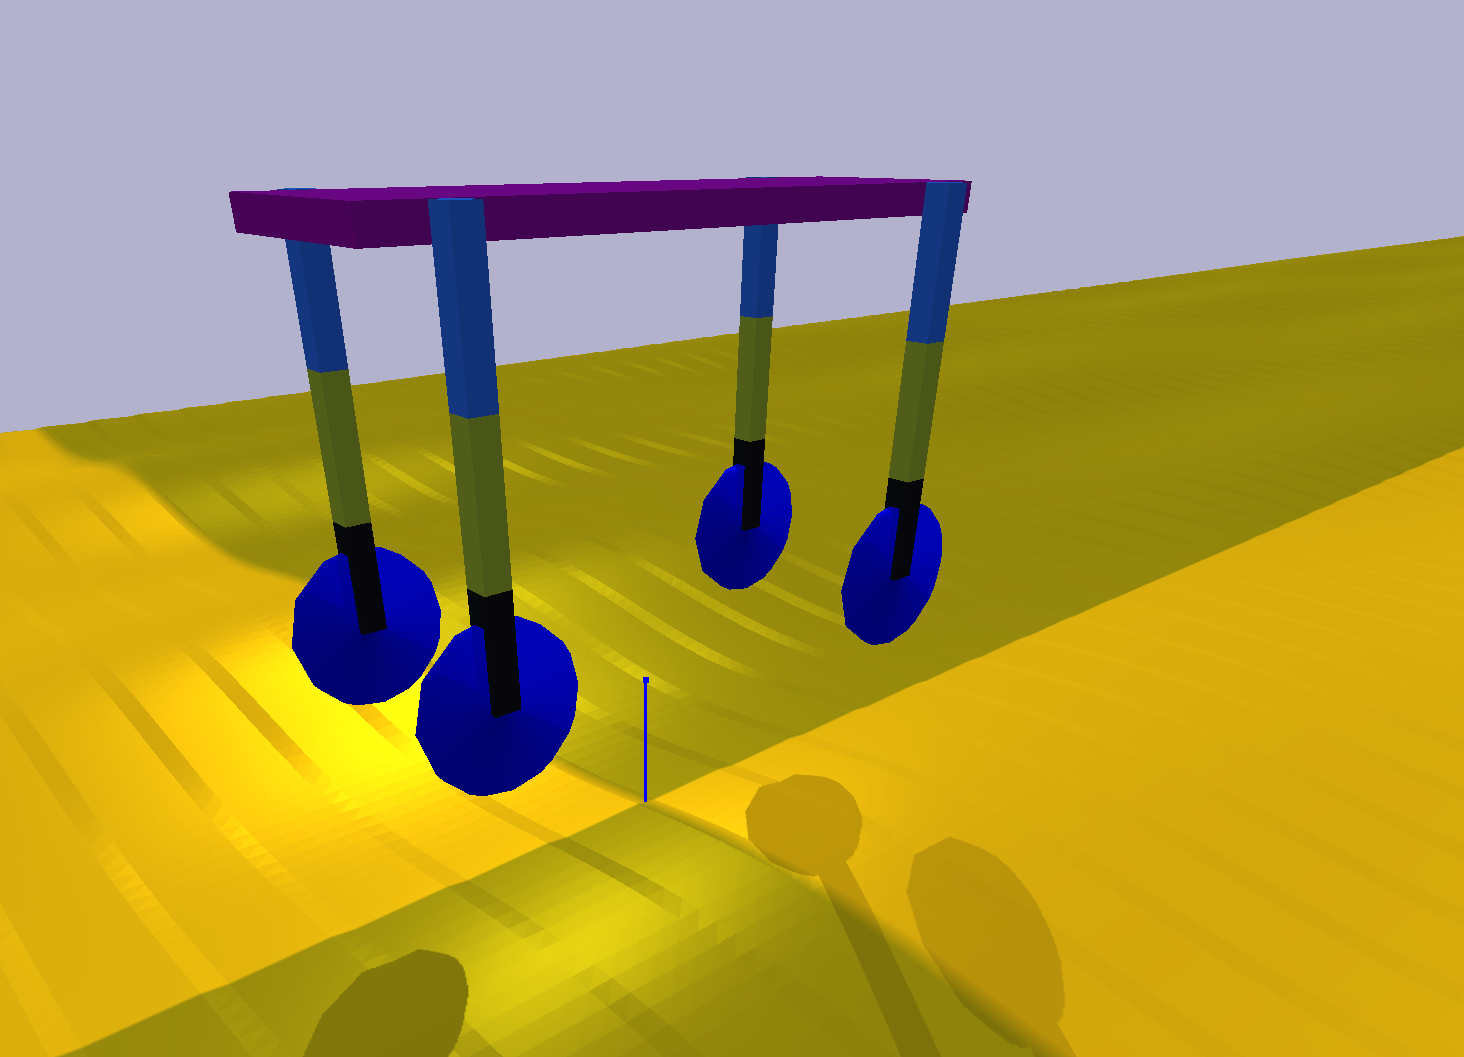
\includegraphics[width=\linewidth]{Figures/ch8_LinearFourWheel.png}
        \caption{Four Wheeler With Linear Actuator}
    \end{subfigure}
    
    \vspace{0.5cm}
    
    \begin{subfigure}[b]{0.45\linewidth}
        \centering
        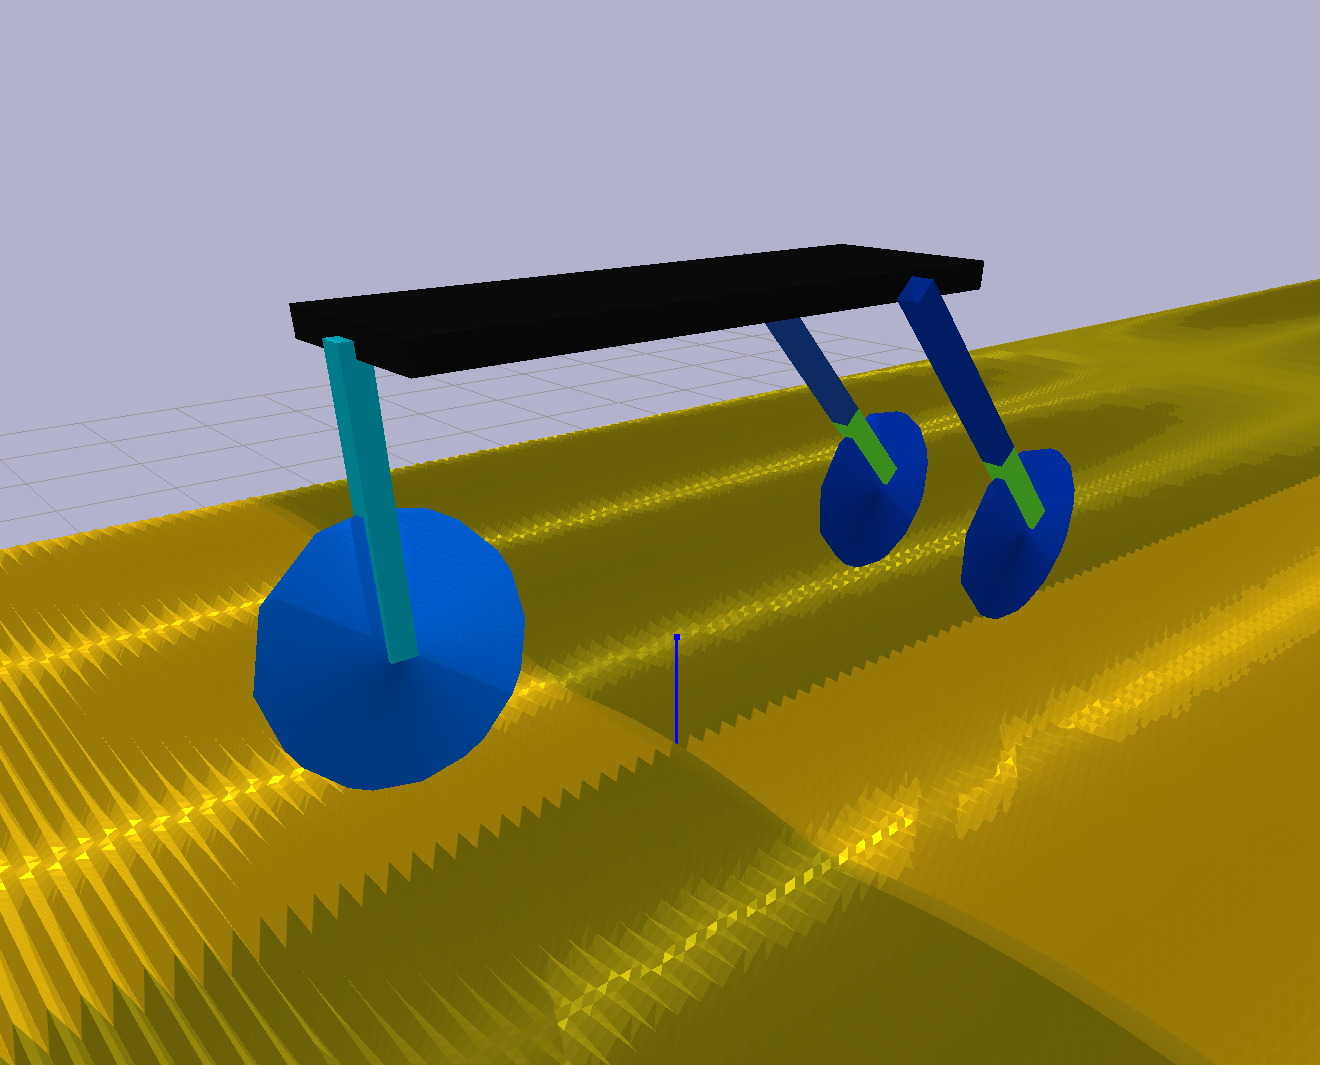
\includegraphics[width=\linewidth]{Figures/ch8_PivotThreeWheel.png}
        \caption{Three Wheeler With Pivot Actuator}
    \end{subfigure}
    \hfill
    \begin{subfigure}[b]{0.45\linewidth}
        \centering
        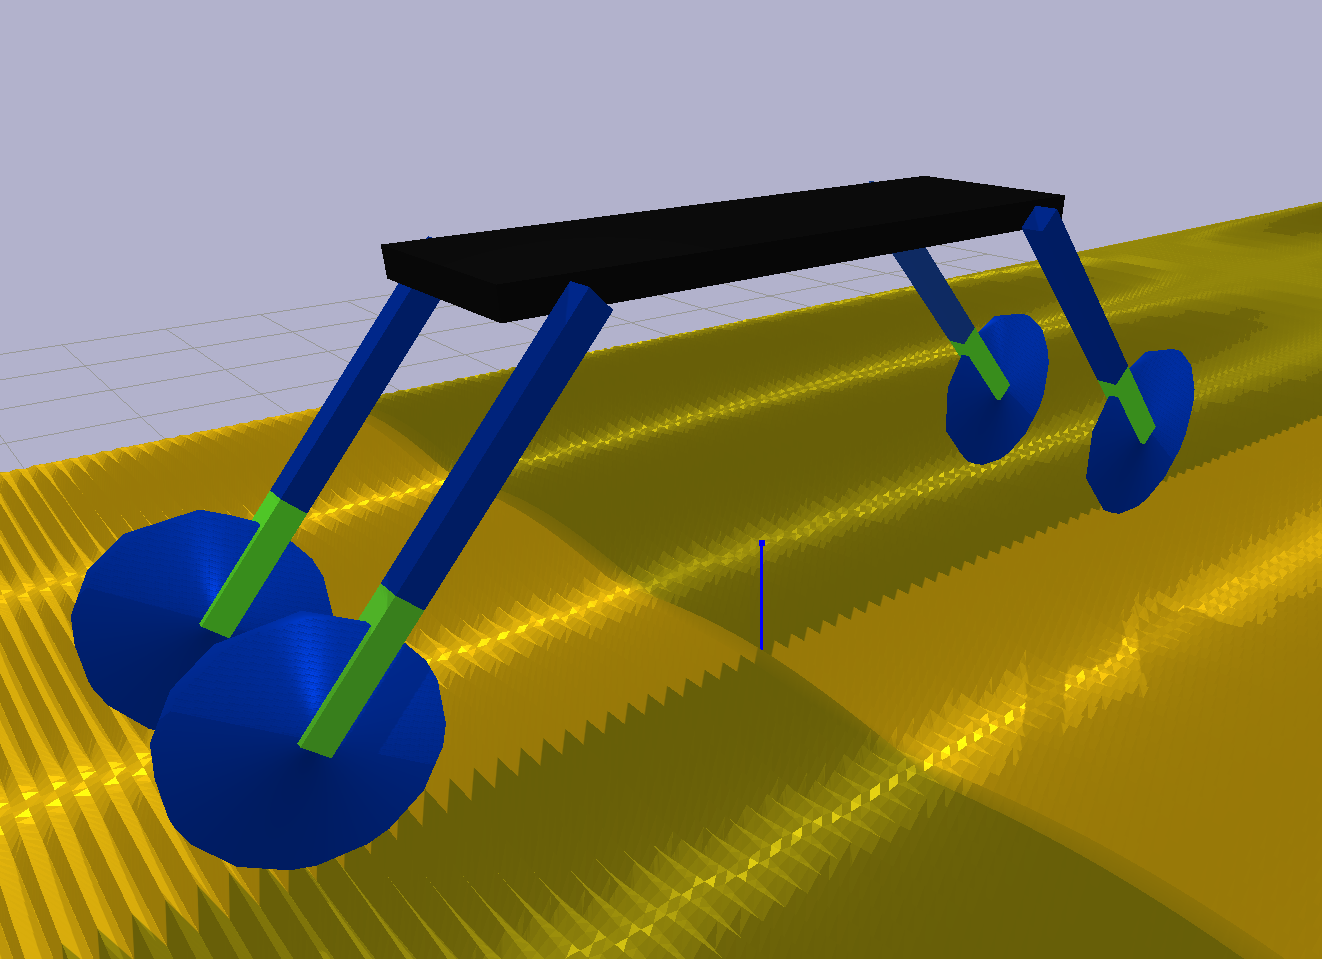
\includegraphics[width=\linewidth]{Figures/ch8_PivotFourWheel.png}
        \caption{Four Wheeler With Pivot Actuator}
    \end{subfigure}
    
    \caption{Comparison of Linear and Pivot Actuated Configurations for Three- and Four-Wheel Designs}
    \label{fig:actuator-configs}
\end{figure}

\subsection{Results}

To assess the dynamic behavior of each configuration, we evaluated their ability to maintain stability under straight-line and constant-radius turning using PID control. Below is a summary of the observed behavior for each of the four combinations of chassis layout (3-wheel vs. 4-wheel) and lean mechanism (pivot vs. linear actuator):

\begin{wrapfigure}{r}{0.45\linewidth}
    \centering
    \vspace{-1em}
    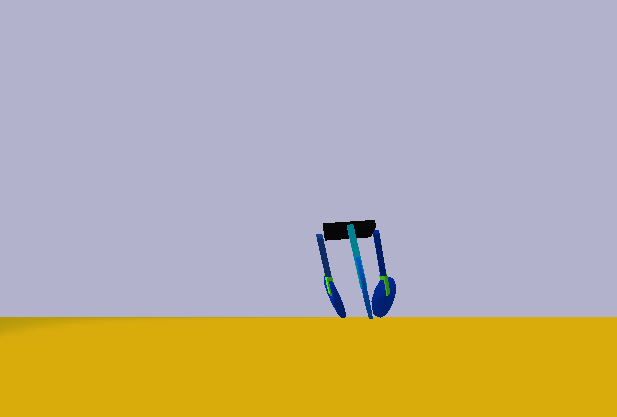
\includegraphics[width=\linewidth]{Figures/ch7_inwardWheel.png}
    \caption{Wheel inward locking behavior in pivot-based designs}
    \label{fig:wheel_instability}
    \vspace{-1em}
\end{wrapfigure}

In the pivot-based configurations, especially the 3-wheel version, we observed a strong tendency for wheels to lock inward or outward due to mass loading, as shown in Figure~\ref{fig:wheel_instability}. This arises from the geometry of the pivot as the mass of the cockpit press on the leg, which find a new minimum by having both wheel going inward or outward. If one try to mitigate the issue by increasing the spring constant of the wheel pivot, the vehicle is not able to turn smoothly and slip instead.

This behavior makes the pivot-based system unsuitable for high-speed or open-loop control. 

Furthermore, For both system, the \textit{mechanical trail} behind the pivot axis improves stability, which is consistent with known self-aligning behaviors in caster-like systems.

Both linear actuator variants (3- and 4-wheel) responded well to PID control in maintaining lean stability. Wheel wobble emerged at high speeds, particularly in the 3-wheel variant, but were manageable with increased damping and should likely be solved with a controller that will impact the wheel speed to create a cancelling moment. Both the three wheel and Four wheel linear actuator variant performed equally well. The four wheel variant as the advantage of allowing the loss of one of the actuator and thus offer some redunduncy. 

Figure~\ref{fig:linear_success_turn} and Figure~\ref{fig:fourwheel_success} show that it's possible to stabilize a steady state turn of the linear actuator based lean control during steady-state turning and straight line driving.

The plot showing the position, speed, acceleration of each element did not yield much result except to help tune the PID by looking at the response.
\begin{figure}[h!]
    \centering
    \begin{subfigure}[b]{0.48\linewidth}
        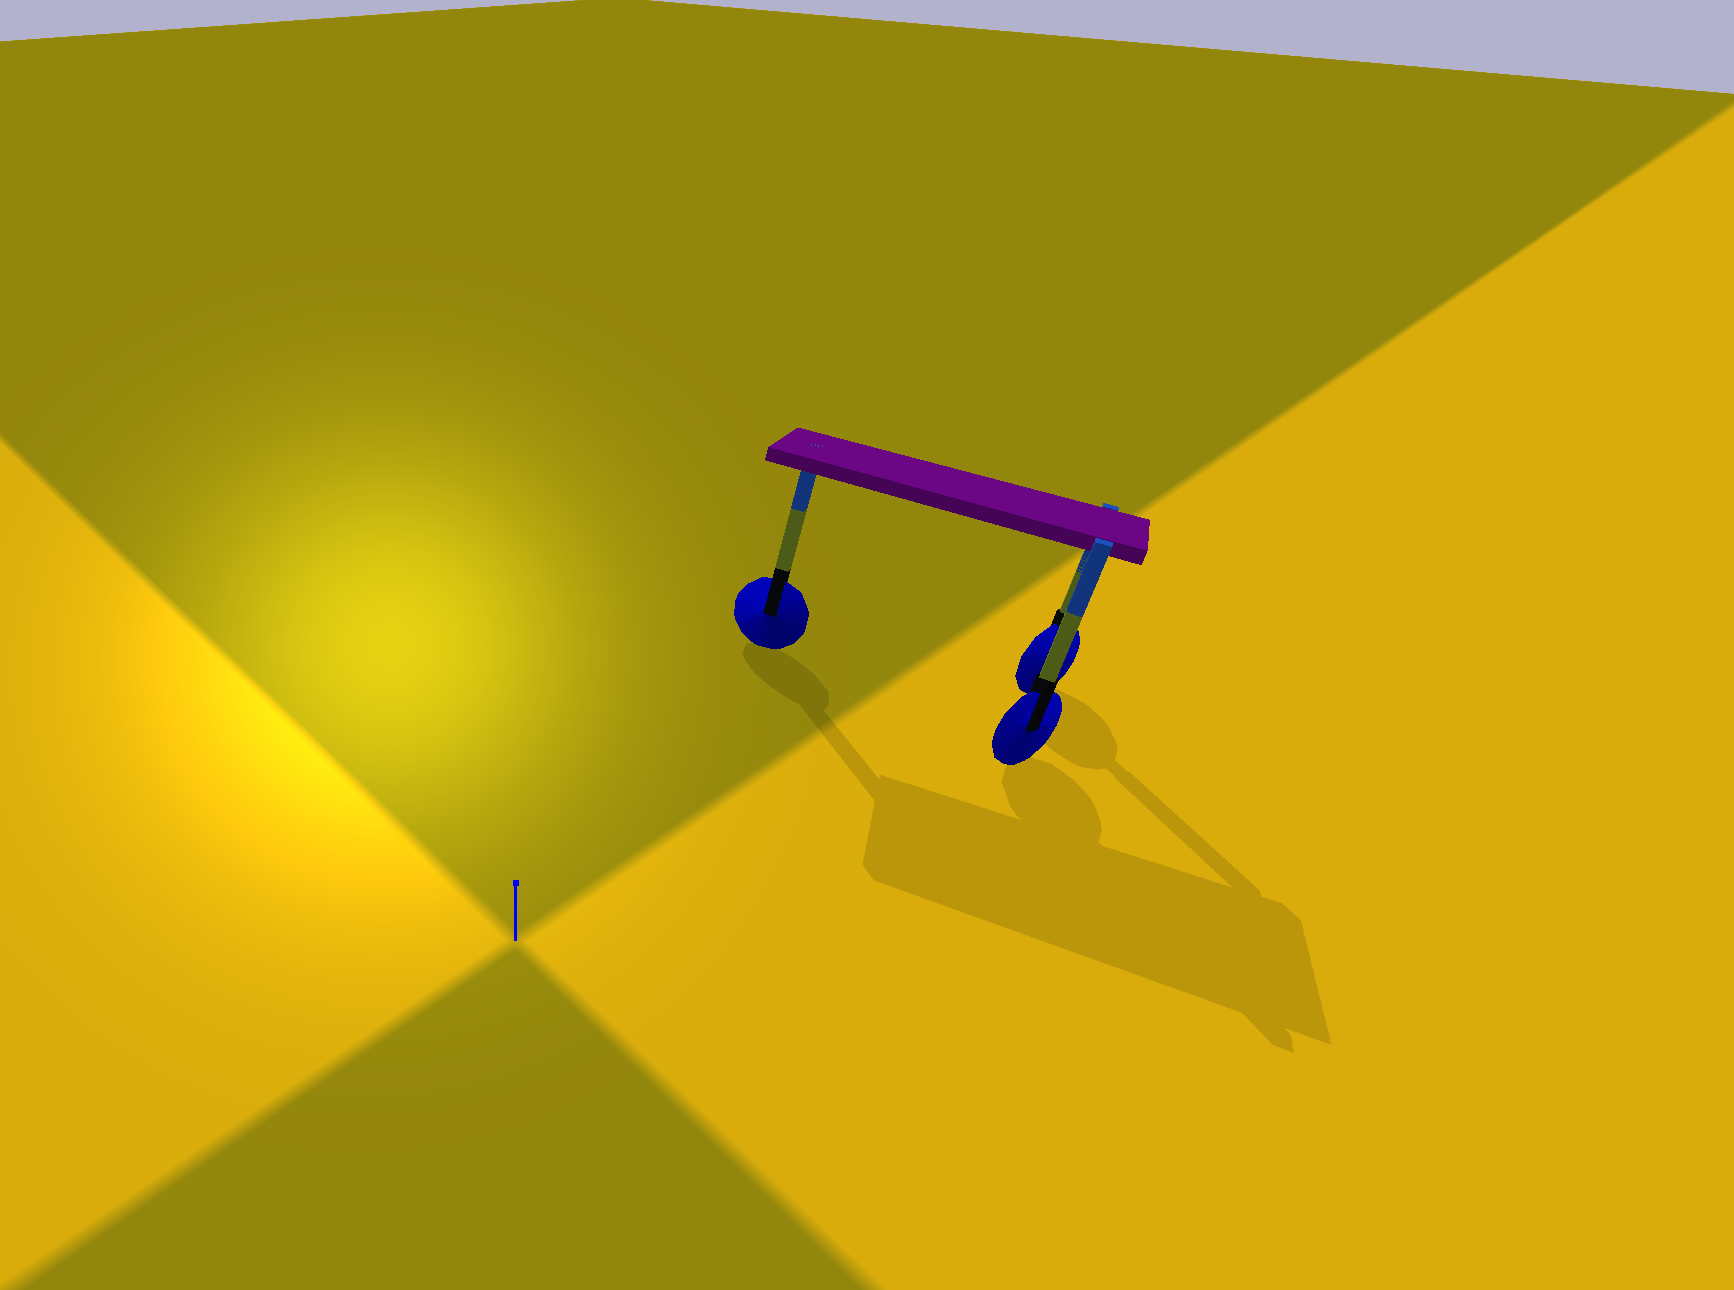
\includegraphics[width=\linewidth]{Figures/ch8_ThreeWheelLinearTurning.png}
        \caption{Three-wheel linear actuator turning}
        \label{fig:linear_success_turn}
    \end{subfigure}
    \hfill
    \begin{subfigure}[b]{0.48\linewidth}
        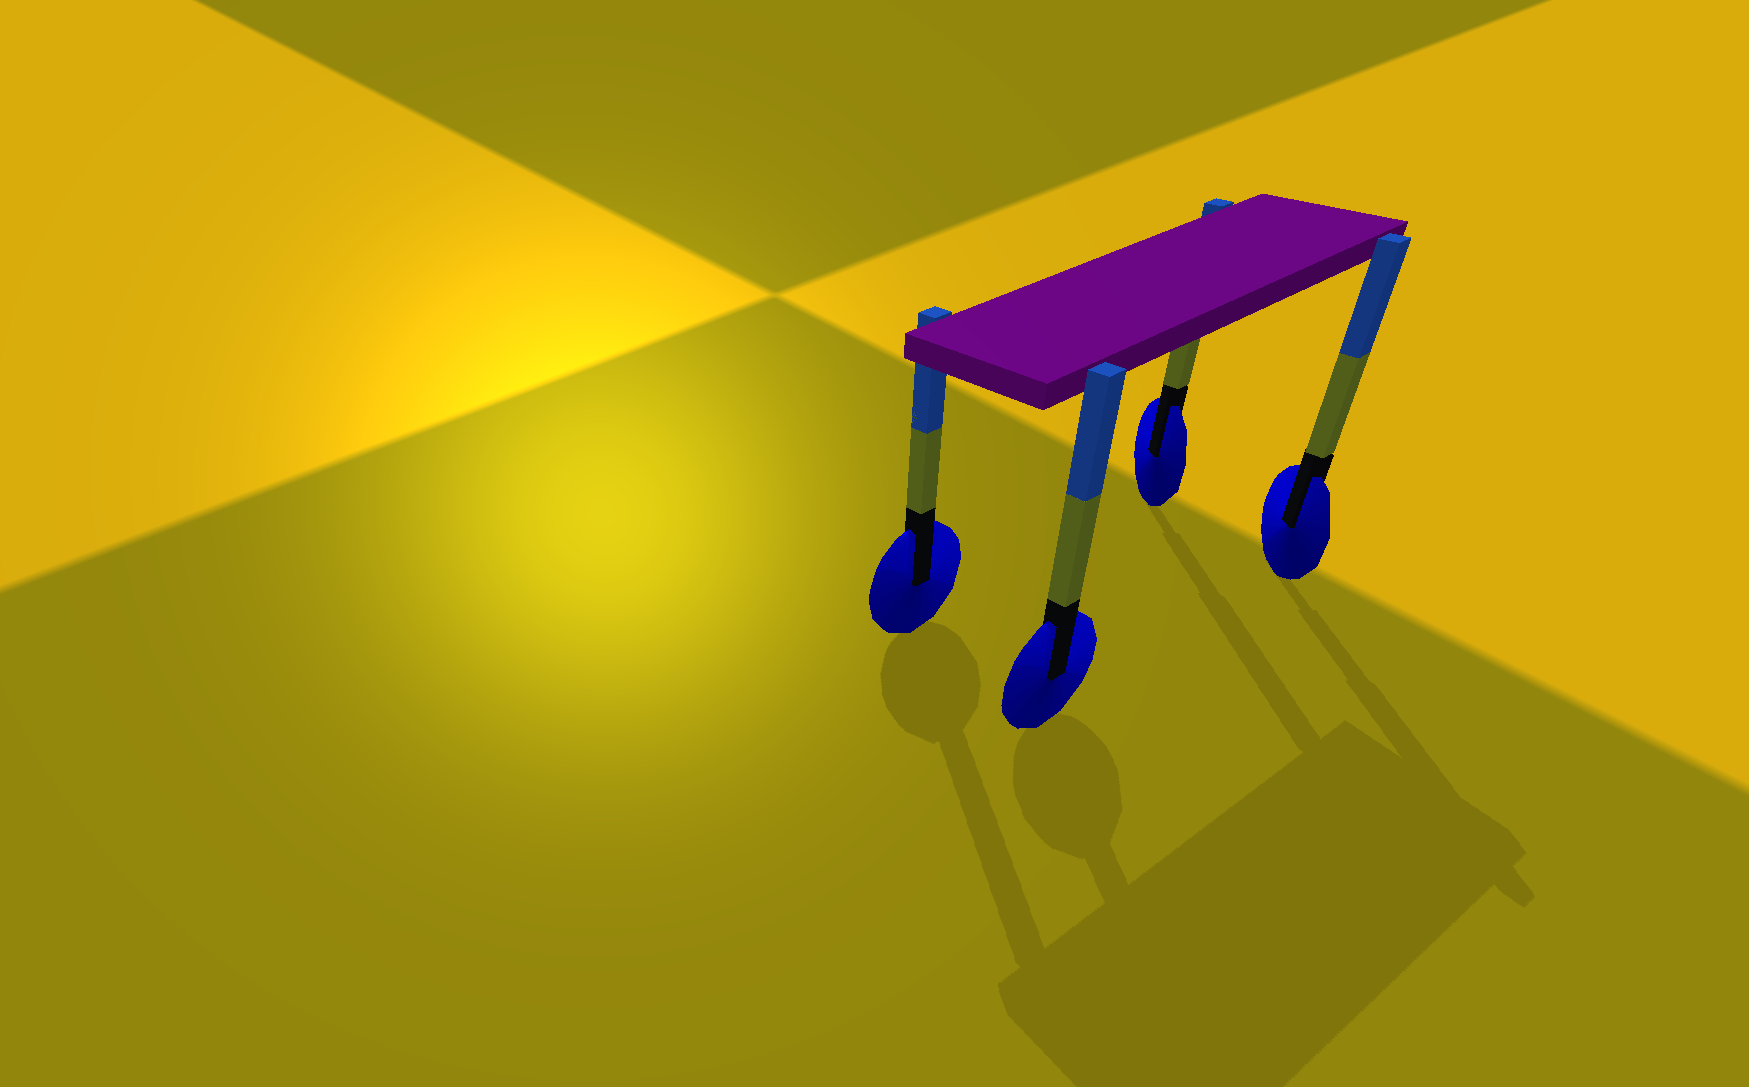
\includegraphics[width=\linewidth]{Figures/ch8_FourWheelSuccessfullTurn.png}
        \caption{Four-wheel linear actuator turning}
        \label{fig:fourwheel_success}
    \end{subfigure}
    \caption{Successful steady-state turning in linear actuator configurations}
\end{figure}

\begin{table}[h!]
\centering
\begin{tabular}{|c|c|c|}
\hline
\textbf{} & \textbf{Pivot Mechanism} & \textbf{Linear Actuator} \\
\hline
\textbf{3-Wheel} & 
\begin{tabular}[c]{@{}l@{}}
- Inherent instability in wheel alignment\\
- Wheels tend to lock inward/outward\\
- Trail effect offers some self-correction\\
- Poor turn stability without speed control
\end{tabular}
&
\begin{tabular}[c]{@{}l@{}}
- Stable under moderate speed\\
- Lean control effective with PID\\
- Wheel oscillation at high speed\\
- Responsive to speed vectoring
\end{tabular}
\\
\hline
\textbf{4-Wheel} & 
\begin{tabular}[c]{@{}l@{}}
- Only 2 passive pivoting wheels allowed\\
- Otherwise becomes uncontrollable\\
- Self-alignment is weak\\
- Strong inward force on wheels
\end{tabular}
& 
\begin{tabular}[c]{@{}l@{}}
- Most stable configuration\\
- Smooth turn response with PID\\
- Capable of steady-state turning\\
- Requires speed differential control
\end{tabular}
\\
\hline
\end{tabular}
\caption{Qualitative behavior observed in the four configurations}
\label{tab:design-summary}
\end{table}

These results suggest that a high-CoM tilting vehicle can be stabilized, provided the mechanical layout don't add too many non-linear coupling and independent wheel speed control is available.
